
\subsection{Enumeration of Explanation}

The enumeration of AXp and CXp can be done with the algorithm in~\cite{MSGCIN20}
and with algorithm Marco~\cite{LiffitonM13}, shown in Algorithm~\ref{alg:marco}.

\begin{algorithm}
    \caption{MARCO algorithm}\label{alg:marco}
    \KwIn{Unsatisfiable constraint set \( C = \{C_1, C_2, C_3, \dots, C_n\} \)}
    \KwOut{MSSes and MUSes of \( C \) as they are discovered}
    $Map \gets \text{BoolFormula}(nvars = |C|)$ \tcp*[r]{Empty formula over $|C|$ Boolean variables}
    \While{$Map$ is satisfiable}{
        $m \gets \text{getModel}(Map)$\;
        $seed \gets \{C_i \in C : m[x_i] = \text{True}\}$ \tcp*[r]{Project the assignment $m$ onto $C$}
        \eIf{$seed$ is satisfiable}{
            $MSS \gets \text{grow}(seed, C)$\;
            \KwYield $MSS$\;
            $Map \gets Map \land \text{blockDown}(MSS)$\;
        }{
            $MUS \gets \text{shrink}(seed, C)$\;
            \KwYield $MUS$\;
            $Map \gets Map \land \text{blockUp}(MUS)$\;
        }
    }
\end{algorithm}

The application of Marco algorithm to enumeration of AXp's and CXp's was 
explained in~\cite{IgnatievNA020}.
There are also algorithms for particular cases, monotonic classifiers~\cite{MarquesSilvaGCIN21} and decision lists~\cite{IgnatievS21}.

We can see how the algorithm works with the following example.

\begin{example}
    Given a set of features $\mathcal{A} = \{x_1, x_2, x_3\}$.
    %
    Let a formula be
    $\phi = (x_1 \land x_2) \lor (x_2 \land x_3)$, 
    and an instance $\mathbf{x} = \{1, 1, 1\}$.
    It's straightforward to see 
    that its AXp's and CXp's are:
    \begin{eqnarray*}
    AXp's &:& \{ 1, 2 \}, \{ 2, 3 \} \\
    CXp's &:& \{1, 3\}, \{2\}
    \end{eqnarray*}

    In  Figure~\ref{fig:lattice1}, the circles correspond to the AXp's, 
    and to the rest of node correspond to the WCXp's. 
    %
    A set in a node represents the set of literals for an WAXP, 
    and the complementary set of literals for a WCXP.
    %
    The AXp's are the minimal points of the set of WAXp's, 
    and the CXp's are the maximal points of the set of WCXp's,
    being the lattice subset-minimal ordered.
    These sets are plotted in the lattice in gray.

    \begin{figure}
        \begin{center}
        
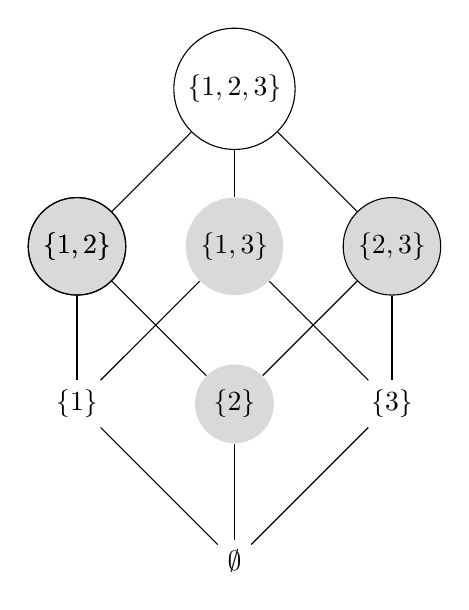
\begin{tikzpicture}%[scale=1.5, transform shape, every node/.style={draw, circle, minimum size=1cm}]
    % Define the subsets
    \node (empty) at (0,0) {$\emptyset$};
    \node (1) at (-2,2) {$\{1\}$};
    \node[circle, minimum size=1cm, fill=gray!30] (2) at (0,2) {$\{2\}$};
    \node (3) at (2,2) {$\{3\}$};
    \node[draw, circle, minimum size=1cm, fill=gray!30] (12) at (-2,4) {$\{1, 2\}$};
    \node[circle, minimum size=1cm, fill=gray!30] (13) at (0,4) {$\{1, 3\}$};
    \node[draw, circle, minimum size=1cm, fill=gray!30] (23) at (2,4) {$\{2, 3\}$};
    \node[draw, circle, minimum size=1cm] (123) at (0,6) {$\{1, 2, 3\}$};
    
    \node[draw, circle, minimum size=1cm] (12) at (-2,4) {$\{1, 2\}$};

    % Draw the edges
    \draw (empty) -- (1);
    \draw (empty) -- (2);
    \draw (empty) -- (3);
    \draw (1) -- (12);
    \draw (1) -- (13);
    \draw (2) -- (12);
    \draw (2) -- (23);
    \draw (3) -- (13);
    \draw (3) -- (23);
    \draw (12) -- (123);
    \draw (13) -- (123);
    \draw (23) -- (123);
\end{tikzpicture}


        \end{center}
    \caption{Lattice for the example.}\label{fig:lattice1}
    \end{figure}

\end{example}
